\documentclass[a4paper]{article}\usepackage[]{graphicx}\usepackage[]{color}
%% maxwidth is the original width if it is less than linewidth
%% otherwise use linewidth (to make sure the graphics do not exceed the margin)
\makeatletter
\def\maxwidth{ %
  \ifdim\Gin@nat@width>\linewidth
    \linewidth
  \else
    \Gin@nat@width
  \fi
}
\makeatother

\definecolor{fgcolor}{rgb}{0.345, 0.345, 0.345}
\newcommand{\hlnum}[1]{\textcolor[rgb]{0.686,0.059,0.569}{#1}}%
\newcommand{\hlstr}[1]{\textcolor[rgb]{0.192,0.494,0.8}{#1}}%
\newcommand{\hlcom}[1]{\textcolor[rgb]{0.678,0.584,0.686}{\textit{#1}}}%
\newcommand{\hlopt}[1]{\textcolor[rgb]{0,0,0}{#1}}%
\newcommand{\hlstd}[1]{\textcolor[rgb]{0.345,0.345,0.345}{#1}}%
\newcommand{\hlkwa}[1]{\textcolor[rgb]{0.161,0.373,0.58}{\textbf{#1}}}%
\newcommand{\hlkwb}[1]{\textcolor[rgb]{0.69,0.353,0.396}{#1}}%
\newcommand{\hlkwc}[1]{\textcolor[rgb]{0.333,0.667,0.333}{#1}}%
\newcommand{\hlkwd}[1]{\textcolor[rgb]{0.737,0.353,0.396}{\textbf{#1}}}%

\usepackage{framed}
\makeatletter
\newenvironment{kframe}{%
 \def\at@end@of@kframe{}%
 \ifinner\ifhmode%
  \def\at@end@of@kframe{\end{minipage}}%
  \begin{minipage}{\columnwidth}%
 \fi\fi%
 \def\FrameCommand##1{\hskip\@totalleftmargin \hskip-\fboxsep
 \colorbox{shadecolor}{##1}\hskip-\fboxsep
     % There is no \\@totalrightmargin, so:
     \hskip-\linewidth \hskip-\@totalleftmargin \hskip\columnwidth}%
 \MakeFramed {\advance\hsize-\width
   \@totalleftmargin\z@ \linewidth\hsize
   \@setminipage}}%
 {\par\unskip\endMakeFramed%
 \at@end@of@kframe}
\makeatother

\definecolor{shadecolor}{rgb}{.97, .97, .97}
\definecolor{messagecolor}{rgb}{0, 0, 0}
\definecolor{warningcolor}{rgb}{1, 0, 1}
\definecolor{errorcolor}{rgb}{1, 0, 0}
\newenvironment{knitrout}{}{} % an empty environment to be redefined in TeX

\usepackage{alltt}

\usepackage[english]{babel}
\usepackage[utf8]{inputenc}
\usepackage{amsmath}
\usepackage{graphicx}
\usepackage[colorinlistoftodos]{todonotes}
\usepackage{float}
\usepackage{natbib}
\usepackage{rotating}
\usepackage{array}
\usepackage{siunitx}
\usepackage{rotfloat}
\usepackage{titling}
\usepackage{booktabs}
\usepackage{amsmath}
\newcommand{\subtitle}[1]{%
  \posttitle{%
    \par\end{center}
    \begin{center}\large#1\end{center}
    \vskip0.5em}%
}
\usepackage{setspace}
\doublespacing

\title{Coercive Diplomacy and the Institutional Consequences of Economic Sanctions} 

\author{Darin Self}

\date{October 8, 2015}
\IfFileExists{upquote.sty}{\usepackage{upquote}}{}
\begin{document}
\bibpunct{(}{)}{;}{a}{}{,} 
\maketitle
\clearpage
\section*{\large{Datasets and Variables}}

The data I use to measure the impact economic sanctions have on target countries is limited largely because economic costs are estimated rather than measured directly. For this study I employ two different datasets used in previous studies to measure costs of economic sanctions. Both datasets build on an original dataset created by \citet[Henceforth \textbf{HSE}]{hufbauer1990economic}. The first is an updated version of HSE that transforms the data into a country-year format (Marinov 2005). The data represent 1,181 cases of economic sanctions from the time-period 1947--1999. In this dataset \citet{marinov2005economic} measures sanctions as a dichotomous variable. \citet{wood2008hand} builds on HSE and \citet{marinov2005economic} by applying a ordinal scale for the level of severity of sanctions. In addition to an ordinal scale of sanctions \citet{wood2008hand} also distinguishes between sanctions levied by the United States or the United Nations. 

\centerline{\textit{Response Variables}}

\par
The purpose of this study is to shed greater light on the effect of exogenous shocks in the form of economic sanctions on democracy. As this is the design of the study, three widely used measures of democracy can be considered; Freedom House, Polity IV, and ACLP.  Previous studies seeking to understand the externalities experienced as a result of economic sanctions focused on the liberal definition of democracy and used the Freedom House measure \cite{lopez1997economic, peksen2009better, peksen2009economic, peksen2010coercive, pdeksen2010coercive, wood2008hand}. As I am more concerned with the institutional stability of democracy than measuring liberal democracy Freedom House is a less appropriate measure of democracy. This may lead to different findings than the aforementioned studies that employed Freedom House but I expect Freedom House and other measures to be correlated. As can be seen in the figure below, the average measure of democracy actually moves in the same direction after the mid-1980s when Freedom House and Polity IV are compared\footnote{Because Polity IV and Freedom House use different scales I multiplied the average Freedom House score for a given year by 5 and took its average $[Avg(FH)]*5$ The Polity measure uses \textit{polity2} from the Polity IV dataset and is scaled by adding 20 $Avg(polity2 +20)$}.  As can be seen in the figure Freedom House and Polity IV are strongly correlated.
\par

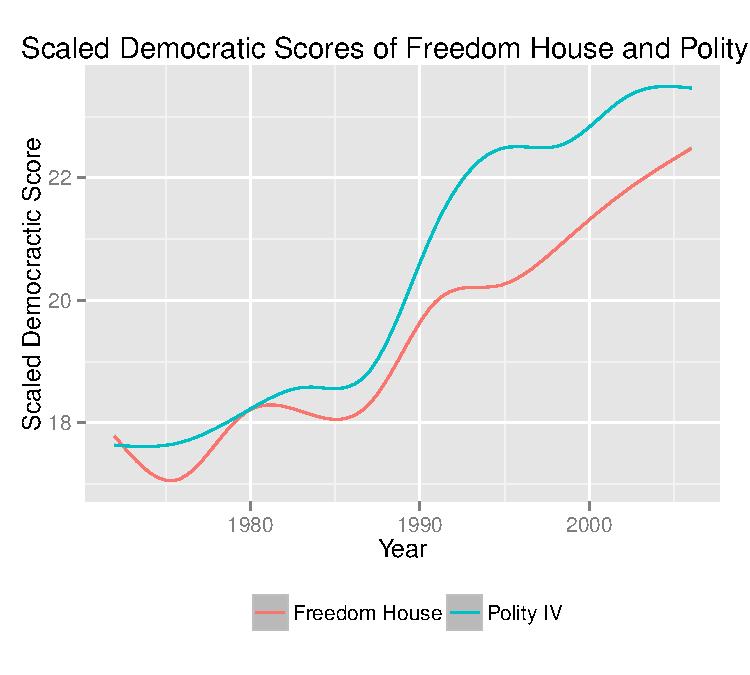
\includegraphics[width=\maxwidth]{figure/unnamed-chunk-1-1} 

\par
The other major dataset used to measure democracy is the dataset created by Pzeworski, Alvarez, Cheibub, and Limongi \citet[Henceforth \textbf{ACLP}]{przeworski2000democracy}. ACLP seeks to measure democracy in an institutional sense but does so with a dichotomous measurement. Within their dataset, Przeworksi et al categorize a regime as either a democracy or a dictatorship. This conceptualization is simplified because of the complexity in operationalizing and measuring democracy and thus, limits the ability to measure more nuanced aspects of democratic institutions such as executive restraint \citep{bogaards2012draw}. Indeed, within ACLP certain regimes are coded as being non-democratic primarily for a lack of transitions of ruling parties, even though elections were mostly free and fair and the executive was institutionally restrained (e.g. Botswana independence to current). The characteristics of the ACLP operationalization of democracy and the use of a dichotomous measure do not identify what I intend to test and are not suitable for this case.  
\par
The other widely used data to measure democracy is Polity IV. Unlike Freedom House, Polity IV codes the level of democracy based on institutional characteristics instead of a normative conception of democracy. In addition, Polity is more nuanced in measuring these characteristics than ACLP. Unlike Freedom House or ACLP Polity IV is measured on a scale of -10 (hereditary monarchy) to + 10 (consolidated democracy). By using a 21-point scale, Polity IV allows me to measure how democratic institutions co-vary with the implementation and severity of sanctions.  
\par
Polity IV is a better measurement of democracy for the purposes of this analysis but it is by no means perfect. Indeed, previous work has shown that the coding of democracy under the Polity IV scheme leads to measurement error. Certain analysis of measures of democracy have found that the measurement error is heteroskedastic for regimes coded on the poles of the Polity scale \citep{treier2008democracy, pemstein2010democratic}. While these problems reduce the power of inference when using Polity it is still deemed to be a superior measure relative to other existing measures of democracy \citep{munck2002conceptualizing} as other measures, such as Unified Democracy Scores, are a synthesis of democracy scores \citep{pemstein2010democratic}.
\par
Despite the cited critiques of the Polity coding scheme it is one of the most, if not the most, reliable measure of democracy available today. Because of the theory developed in the previous section and critiques recently mentioned I will use \textit{polity2} which codes competiveness and openness of executive recruitment, constraints on the executive, regulation and competiveness of participation \citep{marshall2002polity}. 
\par
As previously discussed, I do not expect the covariance of economic sanctions and democracy to be linear. Previous studies that assume a non-linear relationship between Polity IV and another variable have sought to address this problem by delineating Polity IV based on theory. I will seek to do the same in the analysis portion. As discussed in the theory section, I expect the average effect of economic sanctions on democracy to differ between authoritarian regimes (Polity score -10 to -6), competitive authoritarian regimes (Polity score -5 to -2), anocracies (-1 to 1), semi-democracies (2 to 5) and consolidated democracies (6 to 10). The focus will be on regimes that are anocratic \citep{vreeland2008effect, hegre2001toward, fearon2003ethnicity} with the expectation that consolidated regimes are more institutionally consolidated and will not vary with sanctions. While a theoretical delineation of democracy is typically used this demarcation of democracy is unsatisfying.  
\par
A significant critique of the use of Polity IV is that there is no statistical difference between regimes that are coded toward the negative or positive poles (-10 to -8 and 8 to 10)\citep{treier2008democracy}. Because of this issue, I do not believe it is sufficient to demarcate democracy theoretically.  Indeed, I believe because of the error introduced by the human conception of and the latency of democracy, there is a need to identify natural clusters of democracy. In addition to the theoretically derived segments of democracy identified previously, I will use non-parametric partitioning, specifically k-means, to identify clusters of democracy and reduce within group variance. 
\par
\centerline{\textit{Treatment Variables}}
\par
The main explanatory variable that I use to test my hypotheses is \textit{Sanctions}. \textit{Sanctions} is binary measure of sanctions episodes coded by Hufbauer et al. (1990) and later updated by \citet{marinov2005economic}. \textit{Sanctions} is coded as one in the year that sanctions are actually initiated and 0 otherwise. Because the impact of sanctions may be delayed, I test the treatment effect of lagged \textit{Sanctions} on \textit{Regime} in addition to the same-year treatment of \textit{Sanctions}. The dataset is structured as a panel with a dichotomous indicator for whether a state was sanctioned in a given year. 
\\
\centerline{\textit{Control Variables}}
\\
\\
As discussed in the next section I employ a matching method to estimate the effect of sanctions on democracy. I balance the treatment and control groups on a set of variables that help create groups that are balanced on structural characteristics of the state. Namely, I balance on the economic output as measured by the logged GDP as calculated by the UN, logged population size, proportion of economic activity due to industry, and the proportion of the population that resides in urban areas. In addition to these variables, I balance on the size of the rentier state. A rentier effect may allow elites to use resource wealth to avoid the constraints of sanctions and allow these states atypical abilities to skirt the economic hardships induced by sanctions. To balance on the rentier-ness of the state I use a measure of the logged energy production in metric tons of oil \citep{norris2008driving}. Because of a lack of data availability for energy production, industrial output, and level of urbanization I use the \textbf{Amelia} package in R to estimate these values when missing\citep{honaker2011amelia}. 
\section*{\large{Methodology}}
The primary issue in selecting a method to estimate the causal effect of sanctions on democracy is the presence of selection bias. As previously stated many executives have justified the imposition of sanctions because of the democratic characteristics (or lack thereof) of the receiver state. This bias can be illustrated by simply tabulating the average democratic score via Polity IV by whether or not a state was sanctioned. As can be seen in Table 1 states that are sanctioned have a significantly lower Polity IV score than those that are not sanctioned. To address the issue of selection bias I employ multivariate matching to measure the treatment effect of economic sanctions on regime change. 

% Table created by stargazer v.5.1 by Marek Hlavac, Harvard University. E-mail: hlavac at fas.harvard.edu
% Date and time: Wed, Dec 16, 2015 - 12:21:52 AM
\begin{table}[!htbp] \centering 
  \caption{Average Polity IV Score by Dichotomous Lagged Sanction} 
  \label{} 
\begin{tabular}{@{\extracolsep{5pt}} cc} 
\\[-1.8ex]\hline 
\hline \\[-1.8ex] 
Sanction & Regime \\ 
\hline \\[-1.8ex] 
0 & 0.333 \\ 
1 & -1.128 \\ 
\hline \\[-1.8ex] 
\end{tabular} 
\end{table} 

\par
To estimate the effect of sanctions on democracy I used the \textbf{GenMatch} package in R. \textbf{GenMatch} uses genetic matching which is a method employing an evolutionary search algorithm which uses the Mahalanobis distance to balance the data to allow multivariate matching\citep{diamond2013genetic}. When the Mahalanobis distance is not optimal for achieving balance \textbf{GenMatch} searches over the space of distance metrics to find something better. \textbf{GenMatch} generalizes the Mahalanonbis distance by including an additional weight matrix:
\[
d(X_i, X_j) = \left\{ (X_i - X_j)^{T} - (S^{-1/2})^{T} WS^{-1/2}(X_i - X_j)  \right\}^{\frac{1}{2}}
\]
where $W$ is a $k \times k$ positive definite weight matrix and $S^{1/2}$ is the Cholesky decomposition of $S$ which is the variance-covariance matrix of $X$ \citep[pg. 6]{diamond2013genetic}. The balance matrix $X$ supplied for analysis is:

\begin{equation*}
  \begin{aligned}
    X = \{GDP, Population, Energy, Industry, Urban, GDP*Population, \\
     GDP*Energy, GDP*Industry, GDP*Urban, Population*Urban, \\
     Population*Industry, Urban*Industry \}
  \end{aligned}
\end{equation*}

\par
As previously discussed in the data section, I used a non-parametric method, k-means, to determine clusters of democracy which are more probable to change. This was also performed in R using the \textbf{kmeans} command as a method to deliniate democracy. In order to discover the clusters, I used the algorithm on the variables \textit{polity2} and the probability that \textit{polity2} is likely to change given its score for all observations in the dataset. A comparison of the theoretically delineated ranges and the ranges identified non-parametrically are provided in Table 2 below. 
\par




% Table created by stargazer v.5.1 by Marek Hlavac, Harvard University. E-mail: hlavac at fas.harvard.edu
% Date and time: Wed, Dec 16, 2015 - 12:21:52 AM
\begin{table}[!htbp] \centering 
  \caption{Breakdown of Theoretical and Non-parametric Delineation of Democracy Scores} 
  \label{} 
\begin{tabular}{@{\extracolsep{5pt}} cc} 
\\[-1.8ex]\hline 
\hline \\[-1.8ex] 
Theoretical & Non-parametric \\ 
\hline \\[-1.8ex] 
6 to 10 & 8 to 10 \\ 
2 to 5 & 3 to 7 \\ 
-1 to 1 & -2 to 2 \\ 
-5 to -2 & -6 to -3 \\ 
-10 to -6 & -10 to -7 \\ 
\hline \\[-1.8ex] 
\end{tabular} 
\end{table} 

\section*{\large{Results and Discussion}}

To begin estimating the effect of sanctions on democracy I first match \textit{Sanctions} and \textit{Regime} including the full sample of observations on \textit{polity2}. These results are presented in Table 3 below. The primary finding is that, on average, economic sanctions lead to a 1.35 point decrease in \textit{polity2}. This finding is statistically significant and the magnitude of a shift this size under sanctions is substantial. While this is a statistically significant finding it does not reveal much of the impact of sanctions on institutional stability because it is measure the estimated impact of sanctions across the entire Polity IV scale.  To better measure the impact of sanctions on different regime types I estimated the effect of sanctions on regime type across a number of ranges within \textit{polity2} which were delineated both theoretically and non-parametrically. The findings presented in Table 3 actually reject the hypotheses presented earlier. These models suggest that, on average, sanctions are more likely to destabilize regimes closer to consolidated democracies (closer to 10 in \textit{polity2} scale) than regimes in the middle. Further rejecting the proposed hypotheses is the finding that regimes closer to full autocracies (-10 in \textit{polity2}) shift positively under the pressure of sanctions. 
\par
While these findings may immediately reject the hypotheses laid out earlier these findings should be taken with caution. As discussed earlier delineating ranges of regimes using the Polity IV scale could be problematic. By comparing the estimated effect of sanctions on democracy across both the theoretically and non-parametrically delineated ranges of regime we identify sensitivity in the findings. As an example notice the change in the magnitude of the estimated effect for the first range. When this range is theoretically delineated and includes values from 6 to 10 the estimated effect is smaller than a more narrow range of 8 to 10. Again, compare the change in the estimate for the second range in which I delineated regime type from 2 to 5 or 3 to 7. The estimate under a theoretical delineation is double that of the range identified non-parametrically. Similar outcomes are found for the ranges of regime types below full autocracy. In the non-parametrically identified range of -6 to -3 sanctions are found to have a positive substantively large and significant effect on democracy compared to the theoretical range of -5 to -2 where there is no significant finding. 
\par
These findings suggest first that economic sanctions are potentially harmful to regime types that are actually more democratic than autocratic. This rejects the hypotheses laid out earlier. While these results suggest that economic sanctions harm current democracies but push autocracies towards democracy the findings also reveal potential sensitivity in the results. This is best exemplified by the ranges below full autocracies. In the non-parametric case where the range is -6 to -3 there is a substantially large and statistically significant finding. Shift this scale by only positive 1 and this results disappears. Each of these estimates are the results of testing the effect of \textit{Sanctions} on \textit{polity2}

% Table created by stargazer v.5.1 by Marek Hlavac, Harvard University. E-mail: hlavac at fas.harvard.edu
% Date and time: Wed, Dec 16, 2015 - 12:21:52 AM
\begin{table}[!htbp] \centering 
  \caption{Estimated Effect of Economic Sanctions on Democracy} 
  \label{} 
\begin{tabular}{@{\extracolsep{5pt}} ccccccc} 
\\[-1.8ex]\hline 
\hline \\[-1.8ex] 
Delineation & Polity & Estimate & Cases & Matched/Treated Cases & SE & P-Value \\ 
\hline \\[-1.8ex] 
Full Sample & -10 to 10 & $$-$1.35$ & $4,043$ & $797$ & $0.35$ & $0.0001$ \\ 
Theoretical & 6 to 10 & $$-$0.30$ & $1,551$ & $205$ & $0.11$ & $0.01$ \\ 
- & 2 to 5 & $$-$0.21$ & $259$ & $63$ & $0.19$ & $0.27$ \\ 
- & -1 to 1 & $0.11$ & $214$ & $74$ & $0.13$ & $0.41$ \\ 
- & -5 to -2 & $$-$0.03$ & $358$ & $95$ & $0.21$ & $0.88$ \\ 
- & -10 to -6 & $0.33$ & $1,661$ & $360$ & $0.09$ & $0.0003$ \\ 
Non-parametric & 8 to 10 & $$-$0.38$ & $1,218$ & $143$ & $0.10$ & $0.0001$ \\ 
- & 3 to 7 & $$-$0.10$ & $560$ & $122$ & $0.19$ & $0.60$ \\ 
- & -2 to 2 & $0.09$ & $344$ & $98$ & $0.18$ & $0.61$ \\ 
- & -6 to -3 & $0.50$ & $465$ & $120$ & $0.15$ & $0.001$ \\ 
- & -10 to -7 & $0.24$ & $1,456$ & $314$ & $0.08$ & $0.004$ \\ 
\hline \\[-1.8ex] 
\end{tabular} 
\end{table} 

The previous results reported the tests of \textit{Sanctions} on \textit{polity2}. While the findings were surprising there are potential issues with the tests and conclusions should be restrained. One potential issue with these findings is that they estimate the effect of \textit{Sanctions} on \textit{polity2} in the same time period. This potentially exposes the model to simultaneity bias if executives use sanctions to punish receiver states for non-democratic behavior. It is also potentially problematic in that the full effect of sanctions may be delayed. Sanctions take time to implement and their full effect may grow with time. To account for this I effectively run the same estimations as before but estimate the effect of a one-period lag of \textit{Sanctions} on \textit{polity2} \footnote{Using the lag of \textit{Sanctions} resulted in the loss of the first and last observation of each country in the dataset. Because of this I rebalanced the sample for each range of regime type.}. The results are presented in Table 4. 
\par
Estimating the effect of the lag of \textit{Sanctions} on \textit{polity2} leads to a number of different results. The first results, however, is mostly unchanged. For the full sample of countries in the dataset the lag of \textit{Sanctions} has a negative substantially large, albeit slightly smaller, and significant estimated effect on \textit{polity2}. For each sanction imposed this model estimates a one unit negative shift in \textit{polity2} in the year after a sanction is imposed. Unlike the previous models in which \textit{Sanctions} was not lagged the estimates in the upper ranges of \textit{polity2} that are theoretically delineated are not statistically significant. Even though the estimates in these ranges are insignificant this estimation supports that of the non-lagged \textit{Sanctions} in that fully autocratic regimes shift positively under the pressure of sanctions. 
\par
While the estimate of lagged \textit{Sanctions} on \textit{polity2} in the theoretically delineated range of full autocracies (-10 to -6) is similar to the non-lagged treatment there is a significant shift in the non-parametrically delineated ranges. For both of the lower ranges that are identified using a non-parametric strategy there is a statistically weak estimate that a one-unit lag of \textit{Sanctions} leads to a negative shift in \textit{polity2}. This is somewhat surprising for the lowest range considering there is little room to shift negatively. Overall the estimations modeled across the non-parametric ranges of \textit{polity2} do little to support the hypotheses that sanctions will lead to autocratic backsliding in institutionally weak settings. 

% Table created by stargazer v.5.1 by Marek Hlavac, Harvard University. E-mail: hlavac at fas.harvard.edu
% Date and time: Wed, Dec 16, 2015 - 12:21:53 AM
\begin{table}[!htbp] \centering 
  \caption{Estimated Effect of Lagged Economic Sanctions on Democracy} 
  \label{} 
\begin{tabular}{@{\extracolsep{5pt}} ccccccc} 
\\[-1.8ex]\hline 
\hline \\[-1.8ex] 
Delineation & Polity & Estimate & Cases & Matched/Treated Cases & SE & P-Value \\ 
\hline \\[-1.8ex] 
Full Sample & -10 to 10 & $$-$1.09$ & $4,022$ & $769$ & $0.37$ & $0.003$ \\ 
Theoretical & 6 to 10 & $$-$0.08$ & $1,542$ & $202$ & $0.14$ & $0.57$ \\ 
- & 2 to 5 & $$-$0.31$ & $257$ & $68$ & $0.19$ & $0.11$ \\ 
- & -1 to 1 & $0.21$ & $213$ & $71$ & $0.15$ & $0.16$ \\ 
- & -5 to -2 & $$-$0.05$ & $352$ & $86$ & $0.18$ & $0.80$ \\ 
- & -10 to -6 & $0.32$ & $1,658$ & $342$ & $0.10$ & $0.002$ \\ 
Non-parametric & 8 to 10 & $0.39$ & $388$ & $110$ & $0.20$ & $0.05$ \\ 
- & 3 to 7 & $$-$0.17$ & $1,370$ & $176$ & $0.12$ & $0.15$ \\ 
- & -2 to 2 & $$-$0.08$ & $688$ & $104$ & $0.09$ & $0.37$ \\ 
- & -6 to -3 & $$-$0.33$ & $429$ & $94$ & $0.19$ & $0.07$ \\ 
- & -10 to -7 & $$-$0.21$ & $1,147$ & $285$ & $0.11$ & $0.07$ \\ 
\hline \\[-1.8ex] 
\end{tabular} 
\end{table} 

\par
The previous findings reported in Tables 3 and 4 do little to support the stated hypotheses but further investigation is required. Each of these models employ a dichotomous measure of \textit{Sanctions}. This approach assumes that all sanctions are equally damaging to the receiver state. At this point in the empirical exercise I relax this assumption by using a 4 point scale of the strength of sanctions where 0 is no sanction and 3 is a sanction that imposes significant economic harm on the receiver. Because of a lack of power I do not estimate the treatment effect of sanctions at each point of this scale along the ranges of regime type previously analyzed. Instead I must estimate the effect of sanctions on the entire range of \textit{polity2}. I do this using the one-unit lag of \textit{Sanctions} and differentiate between sanctions imposed by the United States and the United Nations. Results are presented in Table 5. 
\par

% Table created by stargazer v.5.1 by Marek Hlavac, Harvard University. E-mail: hlavac at fas.harvard.edu
% Date and time: Wed, Dec 16, 2015 - 12:21:53 AM
\begin{table}[!htbp] \centering 
  \caption{Estimated Effect of (Lagged) U.S. and U.N. Economic Sanctions on Democracy} 
  \label{} 
\begin{tabular}{@{\extracolsep{5pt}} ccccccc} 
\\[-1.8ex]\hline 
\hline \\[-1.8ex] 
Sender & Strength & Estimate & Cases & Matched/Treated Cases & SE & P-Value \\ 
\hline \\[-1.8ex] 
United States & $0$ & $3.74$ & $3,366$ & $2,838$ & $0.91$ & $0.0000$ \\ 
- & $1$ & $0.03$ & $3,366$ & $294$ & $0.53$ & $0.95$ \\ 
- & $2$ & $$-$2.53$ & $3,366$ & $133$ & $0.82$ & $0.002$ \\ 
- & $3$ & $$-$4.72$ & $3,366$ & $101$ & $0.79$ & $0$ \\ 
United Nations & $0$ & $0.63$ & $3,366$ & $3,270$ & $1.09$ & $0.56$ \\ 
- & $1$ & $$-$0.08$ & $3,366$ & $60$ & $0.84$ & $0.92$ \\ 
- & $2$ & $$-$0.35$ & $3,366$ & $20$ & $1.60$ & $0.83$ \\ 
- & $3$ & $$-$2.56$ & $3,366$ & $16$ & $2.19$ & $0.24$ \\ 
\hline \\[-1.8ex] 
\end{tabular} 
\end{table} 

The results reported in Table 6 grant some support for the hypotheses presented earlier. In cases where sanctions imposed by the United States are strong (rating 2 or 3) there is a significant estimated effect of sanctions on \textit{polity2}. Not only are these estimates statistically significant the magnitude of the estimate is simply stunning. In both cases the sanctions are estimated to produce, on average, a negative shift in \textit{polity2} of a least 2.5 points. This effect is unfortunately estimated using the entire range of \textit{polity2} so the ranges where this is substantially and statistically strongest cannot be identified. 
\par 

% Table created by stargazer v.5.1 by Marek Hlavac, Harvard University. E-mail: hlavac at fas.harvard.edu
% Date and time: Wed, Dec 16, 2015 - 12:21:53 AM
\begin{table}[!htbp] \centering 
  \caption{Estimated Effect of (Lagged) U.S. and U.N. Economic Sanctions on Democracy} 
  \label{} 
\begin{tabular}{@{\extracolsep{5pt}} ccccccc} 
\\[-1.8ex]\hline 
\hline \\[-1.8ex] 
Sender & Strength & Estimate & Cases & Matched/Treated Cases & SE & P-Value \\ 
\hline \\[-1.8ex] 
United States & $0$ & $3.74$ & $3,366$ & $2,838$ & $0.91$ & $0.0000$ \\ 
- & $1$ & $0.03$ & $3,366$ & $294$ & $0.53$ & $0.95$ \\ 
- & $2$ & $$-$2.53$ & $3,366$ & $133$ & $0.82$ & $0.002$ \\ 
- & $3$ & $$-$4.72$ & $3,366$ & $101$ & $0.79$ & $0$ \\ 
United Nations & $0$ & $0.63$ & $3,366$ & $3,270$ & $1.09$ & $0.56$ \\ 
- & $1$ & $$-$0.08$ & $3,366$ & $60$ & $0.84$ & $0.92$ \\ 
- & $2$ & $$-$0.35$ & $3,366$ & $20$ & $1.60$ & $0.83$ \\ 
- & $3$ & $$-$2.56$ & $3,366$ & $16$ & $2.19$ & $0.24$ \\ 
\hline \\[-1.8ex] 
\end{tabular} 
\end{table} 


Of particular note these models suggest that sanctions imposed by the United States have a larger, more significant, effect on \textit{polity2} than sanctions imposed by the United Nations independent of their strength. Compared to the United States, where \textit{Sanctions} are strong in the case of the United Nations the effect of \textit{Sanctions} on \textit{polity2} is neither significant nor nearly as large. It should be noted that these findings may be due to a lack of observations. In this data there are far fewer cases of sanctions being imposed by the United Nations. The lack of observations limits our ability to effectively measure the effect of these sanctions on receiver states. 
\par
Even though the lack of observations does not allow me to estimate the effect of different \textit{Sanctions} strengths on \textit{polity2} across both theoretically and non-parametrically delineated ranges of regime I still seek to determine whether the effects estimated and presented in Table 6 hold for both democracies and autocracies. To identify any shift in effects in these two regime types I split the sample into \textit{more democratic} and \textit{more autocratic} regimes. In splitting the sample I remove strong regime types (-10 to -8 and 8 to 10) as these regime types are unlikely to change. I then filter all cases where $polity2 \geq 0$ qualify as \textit{more democratic} and all cases where $polity2 \leq -1$ qualify as \textit{more autocratic}. Using these subsets I again estimate the effect of \textit{Sanctions} on \textit{polity2} and present the results in Table 7. 

% Table created by stargazer v.5.1 by Marek Hlavac, Harvard University. E-mail: hlavac at fas.harvard.edu
% Date and time: Wed, Dec 16, 2015 - 12:21:53 AM
\begin{table}[!htbp] \centering 
  \caption{Estimated Effect of (Lagged) U.S. Economic Sanctions on High and Low Ranges of Democracy} 
  \label{} 
\begin{tabular}{@{\extracolsep{5pt}} ccccccc} 
\\[-1.8ex]\hline 
\hline \\[-1.8ex] 
Polity & Strength & Estimate & Cases & Matched/Treated Cases & SE & P-Value \\ 
\hline \\[-1.8ex] 
0 through 7 & $0$ & $1.83$ & $650$ & $521$ & $0.35$ & $0.0000$ \\ 
- & $1$ & $$-$0.93$ & $650$ & $82$ & $0.34$ & $0.01$ \\ 
- & $2$ & $$-$1.23$ & $650$ & $39$ & $0.44$ & $0.01$ \\ 
- & $3$ & $$-$1.88$ & $650$ & $8$ & $0.85$ & $0.03$ \\ 
-7 through -1 & $0$ & $$-$0.12$ & $1,144$ & $882$ & $0.28$ & $0.67$ \\ 
- & $1$ & $$-$0.32$ & $1,144$ & $127$ & $0.25$ & $0.20$ \\ 
- & $2$ & $0.19$ & $1,144$ & $80$ & $0.44$ & $0.67$ \\ 
- & $3$ & $$-$0.78$ & $1,144$ & $55$ & $0.35$ & $0.02$ \\ 
\hline \\[-1.8ex] 
\end{tabular} 
\end{table} 

\par
The results of these models suggest that the estimated effect of \textit{Sanctions} on \textit{polity2} is stronger and more likely in cases where the receiver state is \textit{more democratic}. In each level of \textit{Sanctions} strength the estimated effect of \textit{Sanctions} on \textit{polity2} is significant and negative. A caveat should be stipulated that the number of cases for \textit{more democratic} are limited and especially limit any inference when \textit{Sanctions} are extremely strong. For cases where receiver states are \textit{more autocratic} the results are more limited. Only in cases where \textit{Sanctions} are extremely strong do we observe any significant result. In these cases the estimate is negative suggesting that only extremely strong \textit{Sanctions} lead to autocratic backsliding in \textit{more autocratic} cases while most sanctions lead to autocratic backsliding in \textit{more democratic} cases. 
\clearpage
\bibliographystyle{chicago}
\bibliography{bib}






\end{document}
